\documentclass[final]{beamer}

\usepackage[size=a0,orientation=portrait,scale=1.2]{beamerposter}
\usepackage[T1]{fontenc}
\usepackage{lmodern}
\usepackage{tcolorbox}
\usepackage{tabularx}
\usepackage{graphicx}
\usepackage{array}
\usepackage{xcolor}
\usepackage{colortbl}
\usepackage{microtype}
\usepackage{amsmath}
\usepackage{tikz}
\usetikzlibrary{arrows.meta,shapes.geometric,positioning}

% ── BYU brand colours ──────────────────────────────────────────────────────────
\definecolor{byuNavy}{HTML}{002E5D}
\definecolor{byuRoyal}{HTML}{0047BA}
\definecolor{byuLightBlue}{HTML}{BDD6E6}
\definecolor{byuOrange}{HTML}{D14124}
\definecolor{byuSlate}{HTML}{7C878E}

% ── Header centering helpers ───────────────────────────────────────────────────
\newlength{\halfpaper}
\setlength{\halfpaper}{0.5\paperwidth}
% Logo x-center = midpoint between text right edge (0.79\paperwidth) and paper right
\newlength{\logox}
\setlength{\logox}{\paperwidth}
\addtolength{\logox}{-0.105\paperwidth}
% Medallion x-center = midpoint between paper left (0) and text left edge (0.21\paperwidth)
\newlength{\medallionx}
\setlength{\medallionx}{0.105\paperwidth}

% ── Direction shorthands ───────────────────────────────────────────────────────
\newcommand{\arnEs}{arn$\rightarrow$es}
\newcommand{\esArn}{es$\rightarrow$arn}
\newcommand{\arnBoth}{arn$\leftrightarrow$es}

% ── Header font sizes ──────────────────────────────────────────────────────────
\newcommand{\headertitlefont}{\fontsize{50}{56}\selectfont\bfseries}
\newcommand{\headerauthorfont}{\fontsize{34}{40}\selectfont}

% ── Inter-box spacing ──────────────────────────────────────────────────────────
\newcommand{\boxsep}{\vspace{1.0em}}

% ── Beamer theme reset ─────────────────────────────────────────────────────────
\usetheme{default}
\setbeamertemplate{navigation symbols}{}
\setbeamertemplate{headline}{}
\setbeamertemplate{frametitle}{}
\setbeamercolor{background canvas}{bg=white}
\setbeamersize{text margin left=0pt,text margin right=0pt}

% ── Footer ─────────────────────────────────────────────────────────────────────
\setbeamercolor{footline}{bg=byuNavy,fg=white}
\setbeamertemplate{footline}{%
  \begin{beamercolorbox}[wd=\paperwidth,ht=3cm,dp=1.5cm,center]{footline}
    {\Large\bfseries AmericasNLP 2026 \textbullet\ ACL 2026}
  \end{beamercolorbox}%
}

% ── tcolorbox styles ───────────────────────────────────────────────────────────
\tcbuselibrary{skins,breakable}
\arrayrulecolor{byuRoyal}

\tcbset{posterbox/.style={
  colframe=byuRoyal, boxrule=2pt, arc=4pt,
  fonttitle=\large\bfseries\color{white},
  colbacktitle=byuRoyal,
  toptitle=4pt, bottomtitle=4pt,
  titlerule=0pt, enhanced,
  before upper={\large\setlength\parskip{0.4em}},
}}

\newtcolorbox{sectionbox}[1]{posterbox,
  colback=white, left=8pt, right=8pt, top=5pt, bottom=4pt, title=#1}

\newtcolorbox{introbox}[1]{posterbox,
  colback=byuLightBlue, left=8pt, right=8pt, top=5pt, bottom=4pt, title=#1}

% Auto-generated by poster/generate_macros.py from results/paper_stats.json
% Do not edit by hand.
\newcommand{\TrainPairs}{55,452}
\newcommand{\NConditions}{8}
\newcommand{\NModels}{48}
\newcommand{\MvcSixHundredArnEs}{43.2}
\newcommand{\MvcThreeBarnEs}{45.8}
\newcommand{\MorfThreeBarnEs}{45.5}
\newcommand{\StdBpeThreeBarnEs}{45.7}
\newcommand{\StdBpeSixHundredArnEs}{43.5}
\newcommand{\VcStdThreeDelta}{0.11}
\newcommand{\VcStdThreePval}{0.340}
\newcommand{\VcOverMorfDelta}{0.33}
\newcommand{\VcOverMorfPval}{0.0012}
\newcommand{\LlmGap}{25+}
\newcommand{\VcBoundariesRemoved}{2,215}
\newcommand{\VcBoundariesTotal}{87,382}
\newcommand{\VcBoundariesRemovedPct}{2.5\%}


\begin{document}
\begin{frame}[t]{}

\vspace{-1.5cm}

% ── HEADER: medallion | centered text | matrix logo ───────────────────────────
\begin{beamercolorbox}[wd=\paperwidth]{headline}
  \begin{tikzpicture}
    \fill[byuNavy] (0,0) rectangle (\paperwidth, 18cm);
    % Left: BYU medallion — centered between poster left edge and title left edge
    \node[anchor=center] at (\medallionx, 9cm)
      {
\includegraphics[height=14cm]{figures/Medallion/medallion_white_navy.pdf}};
    % Right: BYU Matrix Lab logo — centered between text right edge and paper edge
    \node[anchor=center]
      at (\logox, 9cm)
      {
\includegraphics[height=11cm]{figures/matrix_lab_logo.pdf}};
    % Center: titles, authors, affiliation — vertically centered in 18cm header
    \node[anchor=center, text=white, font=\headertitlefont,
          text width=0.58\paperwidth, align=center]
      at (\halfpaper, 13.3cm)
      {Bringing Mapudungun into the Modern MT Ecosystem:};
    \node[anchor=center, text=white, font=\headertitlefont,
          text width=0.58\paperwidth, align=center]
      at (\halfpaper, 9.7cm)
      {Morphology-Aware Tokenization for NLLB-200 Fine-Tuning};
    \node[anchor=center, text=white, font=\headerauthorfont,
          text width=0.58\paperwidth, align=center]
      at (\halfpaper, 6.0cm)
      {Isaac M. Thompson, Brandon M.A. Rogers, Eric K. Ringger};
    \node[anchor=center, text=white!80!byuNavy, font=\headerauthorfont,
          align=center]
      at (\halfpaper, 3.5cm)
      {Brigham Young University \textbullet\ BYU MAchine TRanslation and Interlingual eXperimentation (MATRIX) Lab};
  \end{tikzpicture}
\end{beamercolorbox}

\vspace{0.1cm}

% ── BODY: 1.5% | 47.5% left | 2% gap | 47.5% right | 1.5% ──────────────────
\begin{columns}[t,totalwidth=\paperwidth]

\begin{column}{0.015\paperwidth}\end{column}

%% LEFT COLUMN ─────────────────────────────────────────────────────────────────
\begin{column}{0.475\paperwidth}

\begin{introbox}{Abstract}
\textbf{Mapudungun} (ISO 639-3: \texttt{arn}) is a polysynthetic
language spoken in Chile and Argentina. Our corrected block-aligned training set
contains \TrainPairs{} parallel sentence pairs.

We \textbf{fine-tune NLLB-200} (600M, 1.3B, 3.3B) bidirectionally (\arnBoth)
across \textbf{\NConditions{} tokenization conditions} and introduce
\textbf{Morfessor-VC} (Vocabulary-Constrained), a novel morphological segmentation
method that reduces additional segmentation before NLLB's tokenizer.

\textbf{Key result:} after correcting the Standard BPE runs, it is strongest at
600M and 1.3B. At 3.3B, Standard BPE and Morfessor-VC are statistically tied
($\Delta=\VcStdThreeDelta$, $p=\VcStdThreePval$) on \arnEs{}.
\end{introbox}

\boxsep

\begin{sectionbox}{Language Sample}
A single Mapudungun verb encodes tense, aspect, subject, object, and
negation. The same word tokenizes very differently depending on method
(\texttt{@@} = morpheme boundary, removed at inference):

\vspace{0.4em}
\setlength{\tabcolsep}{7pt}
\renewcommand{\arraystretch}{1.3}
{\large
\begin{tabularx}{\linewidth}{>{\bfseries\color{byuNavy}}l l @{\hspace{1.5em}} l}
\multicolumn{3}{l}{\textit{kutrankautulay}: ``does not become sick''} \\[0.2em]
\multicolumn{3}{l}{kutran (illness) $+$ kautu (to become) $+$ -lay (negation)} \\[0.5em]
\hline\noalign{\vspace{3pt}}
Standard BPE  & \texttt{\_ku tran anka ut ulay} & \\[0.2em]
Morfessor     & \texttt{kutran@@ \textcolor{byuRoyal}{ka@@ u@@} tulay}
              & (spurious \textit{ka+u} split) \\[0.2em]
Morfessor-VC  & \texttt{kutran@@ \textcolor{byuOrange}{kau@@} tulay}
              & (\textit{kau} $\in$ NLLB vocab) \\
\end{tabularx}}
\end{sectionbox}

\boxsep

\begin{sectionbox}{Motivation}
BPE is not designed for polysynthetic morphology. A single Mapudungun
verb can encode tense, aspect, subject, object, evidentiality, and spatial deixis,
inflating \textbf{fertility} (tokens per word) and degrading translation quality.
NLLB-200 does not include Mapudungun: we add \texttt{arn\_Latn} as a new special
token initialized from the mean of three other indigenous Latin-script
languages in NLLB (Aymara, Guaran\'{i}, Quechua).

\vspace{0.3em}
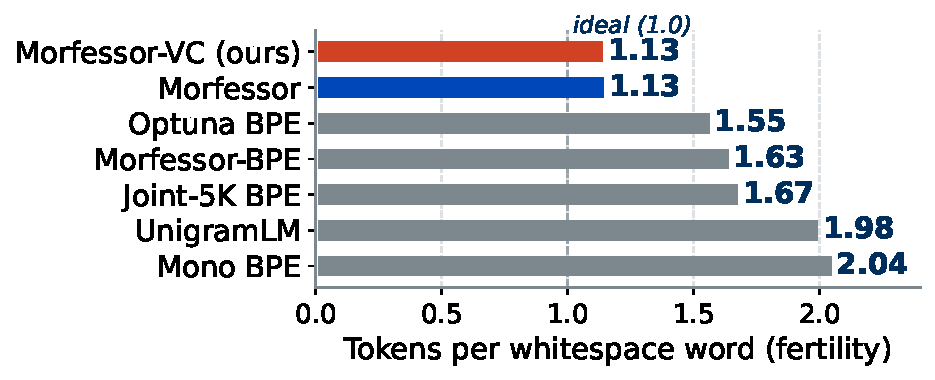
\includegraphics[width=\linewidth]{figures/results_fertility_final.pdf}
{\normalsize\textit{Standard BPE excluded: segmentation is applied internally by
NLLB's tokenizer, making fertility non-comparable.}}

\vspace{0.4em}
\setlength{\tabcolsep}{5pt}
\renewcommand{\arraystretch}{1.2}
{\normalsize
\begin{tabularx}{\linewidth}{|l|>{\raggedright\arraybackslash}X|>{\raggedright\arraybackslash}l|}
\hline
\rowcolor{byuRoyal}
\multicolumn{1}{|c|}{\textcolor{white}{\bfseries Condition}} &
\multicolumn{1}{c|}{\textcolor{white}{\bfseries Description}} &
\multicolumn{1}{c|}{\textcolor{white}{\bfseries Source}} \\ \hline
\bfseries Standard BPE  & NLLB-200 default; segmented internally & (baseline) \\ \hline
\rowcolor{byuLightBlue}\bfseries Morfessor-VC & \bfseries Segment into morphemes; greedily merge adjacent morphemes when their concatenation is in NLLB's vocabulary & \bfseries This paper \\ \hline
\bfseries Morfessor     & Unsupervised morpheme segmentation & Virpioja et al., 2013 \\ \hline
\bfseries Optuna BPE    & Mono BPE with Optuna-tuned vocab size & Akiba et al., 2019 \\ \hline
\bfseries Morfessor-BPE & BPE on Morfessor-segmented text & Banerjee \& Bhattacharyya, 2018 \\ \hline
\bfseries Joint-5K BPE  & Joint arn+es BPE, 5K merges & Duan et al., 2020 \\ \hline
\bfseries UnigramLM     & SentencePiece UnigramLM & Kudo, 2018 \\ \hline
\bfseries Mono BPE      & Monolingual arn BPE, 95\% coverage & Gowda \& May, 2020 \\ \hline
\end{tabularx}}
\end{sectionbox}

\end{column}

\begin{column}{0.02\paperwidth}\end{column}

%% RIGHT COLUMN ────────────────────────────────────────────────────────────────
\begin{column}{0.475\paperwidth}

\begin{sectionbox}{Morfessor-VC (Vocabulary-Constrained)}
Morfessor pre-segmentation adds boundaries before NLLB's internal tokenizer.
Morfessor-VC conservatively removes some of those boundaries using NLLB's
existing vocabulary $V$:

\vspace{0.3em}
\begin{center}
\begin{tikzpicture}[
  box/.style={draw=byuRoyal, fill=white, rounded corners=4pt, font=\normalsize,
              text centered, minimum height=1.0cm, minimum width=2.4cm,
              inner sep=5pt, line width=1.4pt},
  arr/.style={-{Stealth[length=6pt,width=5pt]}, line width=1.4pt, byuNavy},
  lbl/.style={font=\small, color=byuNavy, align=center},
]
  \node[box] (w)  {word};
  \node[box, right=0.65cm of w]  (m)  {Morfessor};
  \node[box, right=0.65cm of m, draw=byuOrange, line width=2pt] (vc) {VC filter};
  \node[box, right=0.65cm of vc] (at) {\texttt{@@} text};
  \node[box, right=0.65cm of at] (n)  {NLLB};
  \node[lbl, below=0.3cm of vc]
    {merge adjacent morphemes when\\their concatenation is in $V$};
  \draw[arr] (w) -- (m);
  \draw[arr] (m) -- (vc);
  \draw[arr] (vc) -- (at);
  \draw[arr] (at) -- (n);
\end{tikzpicture}
\end{center}

\vspace{0.2em}
Given adjacent units $m_i,m_{i+1}$, the greedy left-to-right pass merges them
when $m_i\|m_{i+1}\in V$, then checks the merged unit against the next morpheme.
The method reduces added boundaries; it does not guarantee that every retained
unit is a single NLLB piece.
Of \VcBoundariesTotal{} Morfessor boundaries, only \VcBoundariesRemoved{}
(\VcBoundariesRemovedPct) are removed, so the method is conservative.
\end{sectionbox}

\boxsep

\begin{tcolorbox}[posterbox, colback=white, left=8pt, right=8pt, top=50pt, bottom=45pt, title={\large\bfseries\color{white}Results}]
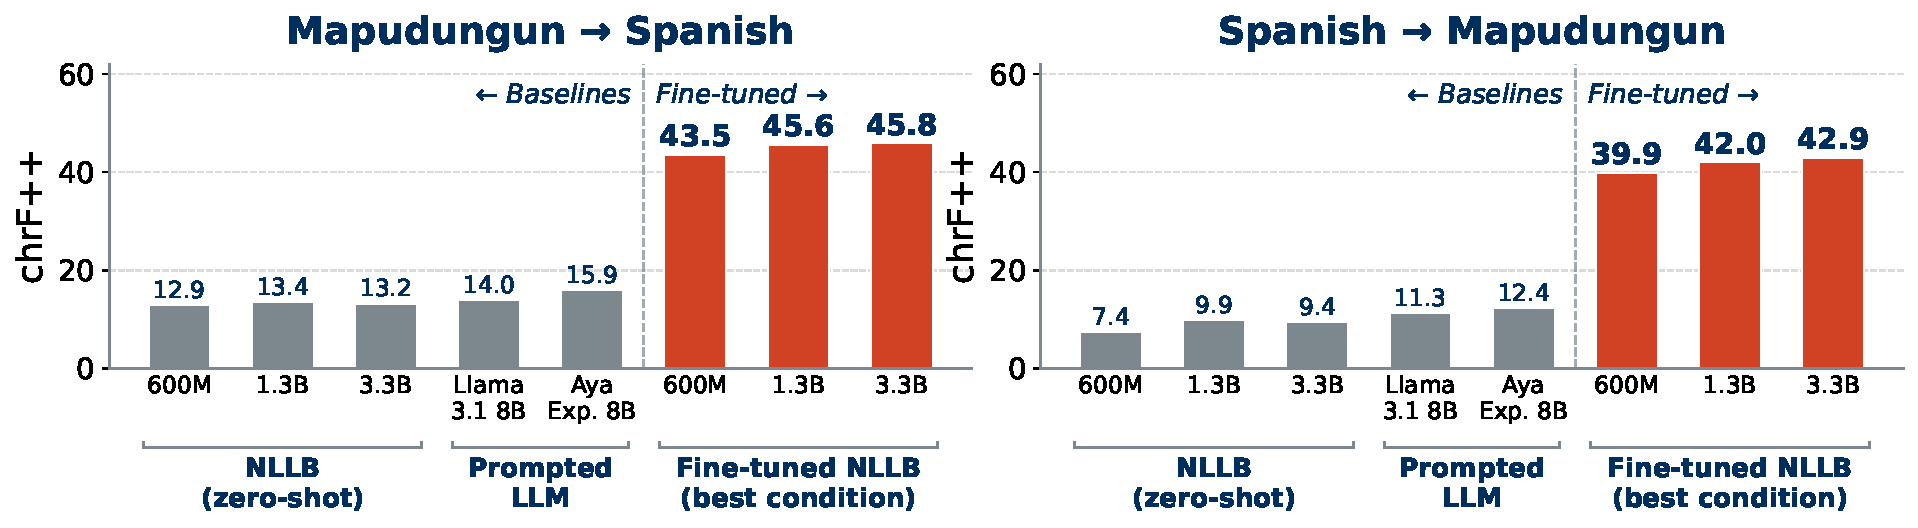
\includegraphics[width=\linewidth]{figures/results_chrf_final.pdf}
\par\vspace*{1.2cm}\par
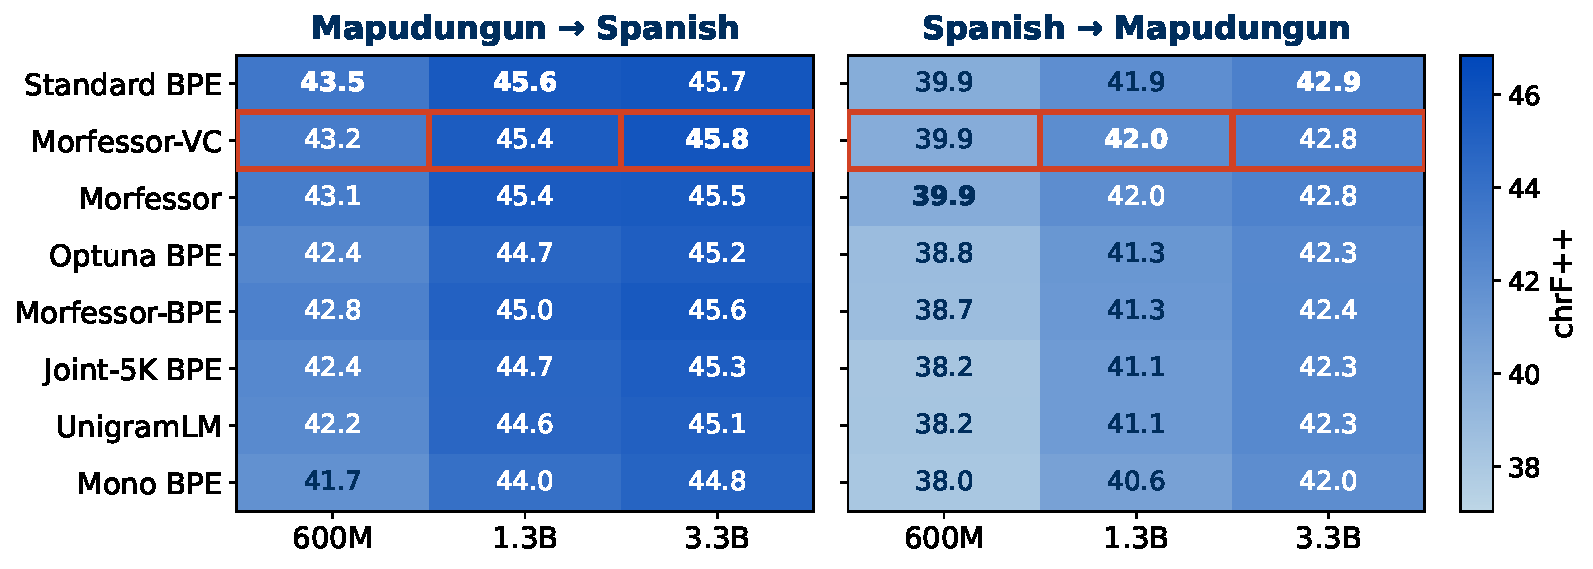
\includegraphics[width=\linewidth]{figures/results_heatmap_final.pdf}
\end{tcolorbox}

\boxsep

\begin{sectionbox}{Key Findings}
\begin{itemize}
  \item Corrected Standard BPE is strongest at 600M and 1.3B; at 3.3B it is
        statistically tied with Morfessor-VC on \arnEs{}.
  \item Morfessor-VC exceeds vanilla Morfessor at 3.3B
        ($\Delta=\VcOverMorfDelta$, $p=\VcOverMorfPval$); the smaller sizes tie or favor Standard BPE.
  \item For \textbf{\esArn}, tokenization has little impact; corpus quality is the
        bottleneck. Future work: larger, cleaner \esArn{} corpora.
  \item All \NModels{} fine-tuned systems surpass the prompted LLM baselines (Llama 3.1 8B,
        Aya Expanse 8B) by \textbf{\LlmGap{} chrF++}.
\end{itemize}
\end{sectionbox}

\boxsep

\begin{sectionbox}{Links}
\setlength\parskip{0pt}%
\noindent\hfill
\begin{minipage}[t]{0.22\linewidth}\centering
  \textbf{Paper (ACL Anthology)}\\[0.3em]
  
\includegraphics[width=3.8cm]{figures/qr_paper.png}\\[0.2em]
  {\scriptsize\ttfamily\shortstack[c]{aclanthology.org/\\[-0.15em]2026.americasnlp-6.16}}
\end{minipage}\hfill
\begin{minipage}[t]{0.22\linewidth}\centering
  \textbf{Repository (GitHub)}\\[0.3em]
  
\includegraphics[width=3.8cm]{figures/qr_github.png}\\[0.2em]
  {\scriptsize\ttfamily\shortstack[c]{github.com/byu-matrix-lab/\\[-0.15em]mapudungun-nllb}}
\end{minipage}\hfill
\begin{minipage}[t]{0.22\linewidth}\centering
  \textbf{Models (HuggingFace)}\\[0.3em]
  
\includegraphics[width=3.8cm]{figures/qr_hf.png}\\[0.2em]
  {\scriptsize\ttfamily\shortstack[c]{hf.co/collections/\\[-0.15em]byumatrixlab/mapudungun-nllb}}
\end{minipage}\hfill
\begin{minipage}[t]{0.22\linewidth}\centering
  \textbf{BYU MATRIX Lab}\\[0.3em]
  
\includegraphics[width=3.8cm]{figures/qr_matrix.png}\\[0.2em]
  {\scriptsize\ttfamily matrix.byu.edu}
\end{minipage}\hfill
\end{sectionbox}

\end{column}

\begin{column}{0.015\paperwidth}\end{column}

\end{columns}

\end{frame}
\end{document}
